\documentclass[review]{elsarticle}

\usepackage{project}

%! Author = sbbfti
%! Date = 10/06/2020

\newacronym{ADF}{ADF test}{Augmented Dickey-Fuller test}
\newacronym{KPSS}{KPSS test}{Kwiatkowski-Phillips-Schmidt-Shin test}
\newacronym{ACF}{ACF}{AutoCorrelation function}
\newacronym{PACF}{PACF}{Partial AutoCorrelation function}


\newacronym{ti}{$T_{i}$}{indoor air temperature, $^{\circ}$C}


\begin{document}
\section{A close relationship between Time Series Classification and Deep Learning }

During the last two decades, time-series classifications have been considered as one of the most challenging problems in data mining (Yang and Wu, 2006; Esling and Agon, 2012). With the increase of temporal data availability, hundreds of time-series algorithms have been proposed since 2015 (Bagnal et al., 2017). Due to natural temporal ordering, time-series data are present in almost every task that requires some sort of human cognitive process (Langkvist et al., 2014). In fact, any classification problem, using data that is registered taking into account some notion of order, can be cast as a time series classification problem (TSC) (Cristian Borges Gamboa, 2017). After having established the current state-of-the-art of non-deep classifiers for TSC (Bagnall et al., 2017) we discuss the success of Deep Learning (LeCun et al., 2015) in various classification tasks which motivated the recent utilization of Deep learning models for TSC(Wang et al., 2017b). Deep Convolutional Neural networks (CNNs) have revolutionized the field of computer vision. There are several classification models including logistic regression, decision tree, random forest, gradient-boosted tree, etc. All these algorithms require some kind of feature engineering as a separate task before the classification is performed, and this can imply the loss of some information and the increase of the development time.  On the contrary, deep learning models already incorporate this kind of feature engineering internally, optimizing it and eliminating the need to do it manually. Therefore, they can extract information from the time series in a faster, more direct, and more complete way. Fig? represent the difference between classic ML algorithms and the deep learning model. 


\subsection{Deep learning}

Figure \ref{fig:a1} shows a general Deep Learning framework for time series classification. It is a composition of several layers that implement non-linear functions. The input is a multivariate time series., Univariate and multivariate time series are two types of data that varying over time, Every layer takes as input the output of the previous layer and applies its non-linear transformation to compute its own output.
In this research, 3 different Deep Learning architectures for time series classifications are presented, called Convolutional neural network, Inception time, and Echo State Network. 



\begin{figure}
    \centering
    \begin{minipage}[b]{.5\textwidth}
        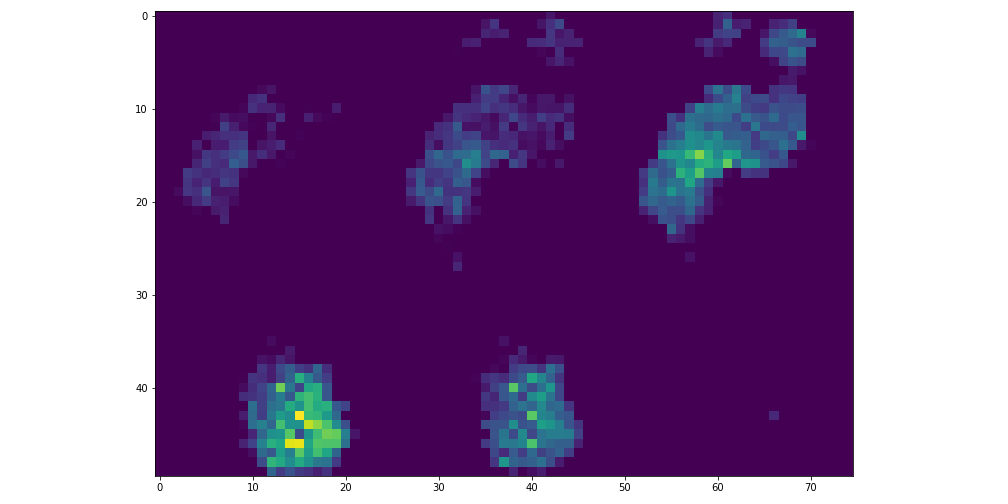
\includegraphics[width=\textwidth]{figures/project/frame1.png}
    \end{minipage}
    \caption{sample image.}
    \label{fig:a1}
\end{figure}

\subsection{Convolutional Neural Networks, that is the most classical and used architecture for time series classifications problems}
Since AlexNet (Krizhevsky et al., 2012) won the imageNet competition in 2012, deep CNNs have seen a lot of successful applications in many different domains (LeCun et al., 2015) such as reaching human-level performance in image recognition problems (Szegedy et al., 2015) as well as different natural language processing tasks (Sutskever et al., 2014; Bahdanau et al., 2015). Motivated by the success of these CNN architectures in these various domains, researchers have started adopting them for time series analysis (Cristian Borges Gambola, 2017).  
A convolutional Neural Network is a deep learning algorithm that takes as input an image or a multivariate time series, is able to successfully capture the spatial and temporal patterns through the application trainable filters and assigns importance to these patterns using trainable weights. The pre-processing required in a Convolutional neural network is much lower as compared to other classification algorithms. While in many methods filters are hand-engineered, the convolutional neural network could learn these filters. Figure? shows the structure of the mentioned algorithm. 

As you observe in the figure ? after several convolution and pooling operations, the original time series is represented by a series of feature maps. All these feature maps are flattened into a column vector, which is the final representation of the original input multivariate time series. The flattened column is connected to the Multi-Layer Perceptron, whose output has several neurons equal to the number of possible classes. 
Backpropagation is applied to every iteration of training. Over a series of epochs, the model can distinguish the input time series thanks to their dominant high-level features and classify them. 


\subsection{Inception Time, that is a new architecture based on Convolutional Neural Networks }
Recently was introduced a deep Convolutional Neural Network called Inception Time. This kind of network shows high accuracy and scalability. As shown in the figure? , the Inception Network consists of a series of Inception Modules followed by a Global Average Pooling Layer and a Fully Connected Layer (usually a Multi-Layer Perceptron). Moreover, a residual connection is added at every third inception module. Each residual block’s input is transferred via a shortcut linear connection to be added to the next block’s input, thus mitigating the vanishing gradient problem by allowing a direct flow of the gradient.

\subsection{Echo State Networks, that is another recent architecture, based on Recurrent Neural Networks }
Echo State Networks are a type of Recurrent Neural Network. Hence it can be useful to have a small introduction about them. Recurrent Neural Networks are networks of neuron-like nodes organized into successive layers, with an architecture similar to one of the standard Neural Networks. In fact, like in standard Neural Networks, neurons are divided into the input layer, hidden layers and output layers. Each connection between neurons has a corresponding trainable weight.  

As has shown in the figure? , the architecture of an Echo State Network consists of an Input Layer, a hidden Layer called Reservoir, a Dimension Reduction Layer, a Fully Connected Layer called Readout, and an Output Layer.
In general, the main difficulty in using CNNs is that they are very dependent on the size and quality of the training data. To solve this problem, many new algorithms were recently elaborated, and among these Inception Time and Echo State Networks perform better than the others. 

Inception Time, fig?  is derived from Convolution Neural Networks and speeds up the training process using an efficient dimension reduction in the most important building block, the Inception Module. Echo State Networks are really helpful to handle chaotic time series. 

Hence, in conclusion, high accuracy and high scalability make these new architectures the perfect candidate for product development.

 \end{document}
